\textit{Activity Model} é estruturado sobre uma linguagem de descrição conhecido por \textit{ACTIVITY-DL}. Um dos elementos dessa linguagem é baseado na álgebra de Allen's que tem como por finalidade definir raciocínios temporais \cite{allenalgebric}. 
As relações definidas por essa álgebra é dada por; 

\begin{enumerate}
	\item $X < Y$ onde $X$: ocorre antes de $Y$ 
	\item $X m Y$,$Y mi X$: $X$ encontra $Y$
	\item $X o Y$, $X oi Y$: $X$ sobrepõem a $Y$
	\item $X s Y$, $Y si X$: $X$ começa $Y$
	\item $X d Y$, $Y di X$: $X$ ocorre durante $Y$	  
	\item $X f Y$, $Y fi X$: $X$ termina junto com $Y$	  	
	\item $X = Y$ $X$ é igual a $Y$	  		
\end{enumerate}

A \textit{Activity Model} define construtores que são semanticamente equivalente a certos operadores da álgebra de Allen's. Esses construtores (atuantes sobre atividades) são definidos pela tabela \ref{acticonstruct}

\begin{table}[H]
\centering
\begin{tabular}{|l|l|l|}
\hline
Construtor & Nome         & Relações de Allen \\ \hline
IND        & Independent  & $A \{ <,>,m,mi,o,oi,s,si,d,di,f,fi,= \} B$\\ \hline
SEQ        & Sequential   & $A \{ <,>,m,mi \} B$\\ \hline
SEQ-ORD    & Ordered      & $A \{ <,>,m \} B$\\ \hline
PAR        & Parallel     & $A \{ o,oi,s,si,d,di,f,fi,= \} B$ \\ \hline
PAR-SIM    & Simultaneous & $A \{ = \} B$\\ \hline
PAR-START  & Start        & $A \{ s,si,= \} B$\\ \hline
PAR-END    & End          & $A \{ f,fi,= \} B$ \\ \hline
\end{tabular}
\caption{Construtores da linguagem \textit{ACTIVITY-DL} \cite{v3sframework}}
\label{acticonstruct}
\end{table}

As relações temporais entre as sub-atividades são especificadas por intermédio de construtores que são formalmente definidos no estudo \cite{allenalgebric}. Essas relações são intermediadas pelo vocábulo \textit{Pré-condição} que tem como por propósito apresentar o contexto sobre qual uma dada atividade deve ser executada. A tabela \ref{precondition} apresenta esses contextos.

\begin{table}[H]
\begin{tabular}{|l|l|p{0.6\linewidth}|}
\hline
\textbf{Categoria} & \textbf{Pré-condição} & \textbf{Descrição}                                                                                                                                                                                                                                              \\ \hline
Condições para perceber  & Nomológico            & Descreve o estado do mundo necessário para que a tarefa seja fisicamente realizável. Condições dependem diretamente das regras de ação definidas no modelo de domínio. Exemplo: Abre a porta se estiver fechada.                                                \\ \hline
Condições para perceber  & Regulamentar          & Descreve o estudo do mundo necessário para uma boa realização da atividade de acordo com prescrito em procedimento. Exemplo: Para desconectar o tubo, a proteções devem ser desgastado.                                                                         \\ \hline
Condições para  Examinar & Contextual            & Descreve o estado de mundo em que a atividade é relevante. Quando essa condição é falsa, então a atividade deve ser ignorada. Exemplo: Limpar o tubo é relevante apenas se o tubo estiver sujo.                                                                 \\ \hline
Condições para  Examinar & Favorável             & Descreve o estado de mundo onde a tarefa é preferencial sobre as demais. Essas condições ajudam a escolher entre várias tarefas quando existe uma alternativa para a realização de uma tarefa decomposta. Exemplo: se o parafuso estiver enferrujado, desarmar. \\ \hline
\end{tabular}
\caption{As pré-condições possíveis para as atividades \cite{v3sframework}}
\label{precondition}
\end{table}


No que tange a questões referentes a segurança e violação, a linguagem \textit{ACTIVITY-DL} deve lidar com atividades em estados de alta degradação bem como com compromissos cognitivos  que são um grande potencial para a geração de risco. Essa condição possibilita a verificação de erros nos seguintes aspectos: atividades de aprendizagem e demonstração de comportamentos similares tendo como base personagens virtuais \cite{v3sframework}. Por conta disso, a linguagem \textit{ACTIVITY-DL} incorpora os conceitos de BCTUs e BATUs cujos fundamentos científicos estão descritos em \ref{risksec}. Ambas tags trabalham com o fato de que, ao menos em partes, o profissional decide por cometer uma dada violação tendo em vista a inviabilidade (ou por não ser prático) efetuar a ação com base no que é definido pelos manuais. 

\textit{Risk Models} é a parte do modelo que define a análise de risco. Existe duas categorias; risco de análise clássico e método de análise de confiabilidade humana. A primeira categoria permite definir uma análise quantitativa de risco, contudo falha ao definir a complexidade dos resultados frente a fatores humanos. Em contrapartida, a segunda categoria considera fatores humanos, contudo falha em definir medidas objetivas sobre questões de segurança \cite{v3sframework}. O \textit{V3S} combina ambas situações usando a abordagem MELISSA \cite{melissaproject} \cite{v3sframework}. Essa abordagem é baseada em três pontos (1) atividades relacionadas em cenários de acidentes, (2) descrição das tarefas de representação e (3) fatores influentes em potencial nas atividades. MELISSA representa os cenário de acidente por meio do gráfico \textit{Bowtie}. Isso consiste na identificação de todos os cenários de acidentes bem como no provisionamento e uma listagem de barreiras para os mesmos. O risco aceitável consiste em escolhas que verificam o número e desempenho dessas barreiras. Os ponto central do gráfico de \textit{Bowtie} consiste em eventos críticos, a parte a esquerda desse gráfico implica as causas do evento e a parte direita do mesmo corresponde as consequências do evento \cite{v3sframework}, \cite{melissaproject}. Essa descrição pode ser analisada na figura \ref{bowtiegraf}. 


\begin{figure}[H]
  \centering
  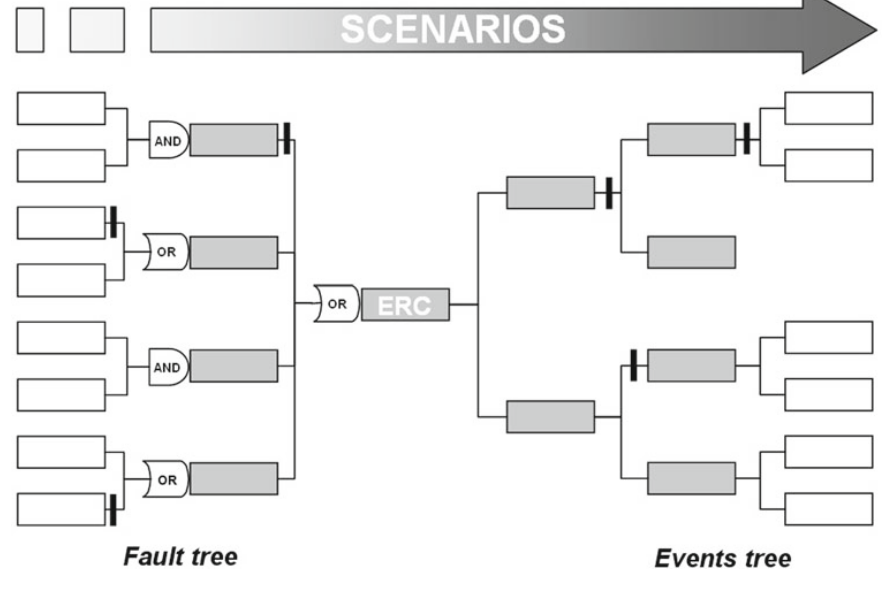
\includegraphics[width=0.5\linewidth]{figure/bowtie.png} 
  \caption{Gráfico de BowTie do texto \cite{melissaproject}}
  \label{bowtiegraf}
\end{figure}


Com o propósito de gerar reflexões no que tange aos riscos de dada atividade, o \textit{V3S} trabalha com o conceito de personagens virtuais em um ambiente. Os raciocínios a cerca destes personagens são feitos usando um formalismo matemático denominado por redes de Petri, ou - mais especificamente máquinas de estado \cite{v3sframework} tendo como base simular a complexidade, flexibilidade e variabilidade de comportamentos que podem ser verificados em um ser humano. Por conta disso, os cientistas desse estudo decidiram modelar esse comportamento usando sistemas multi-agentes, mas especificamente um \textit{framework} conhecido como MASVERP (tratado na seção \ref{agent}).

O \textit{V3S} tem como por finalidade providenciar um modelo que seja coerente, relevante, variado e eficiente em termos de cenário de treinamento com a finalidade de proporcionar atividades de aprendizagem. Esse modelo também apresenta um módulo que monitora cenários adaptativos conhecidos por \textit{HERA}.Em vez de interromper o usuário de forma sistemática a fim de explicar os erros dele, o framework possibilita que o agente cometa erros e observe suas respectivas consequências no mundo virtual. Portanto, a dinâmica do cenário adaptativo permite trazer situações de treinamento relevantes. 

\textit{HERA}, por intermédio de regras baseadas em modelos pedagógicos, fornece o respaldo ao instrutor. Esse retorno é feito por intermédio dos seguintes critérios pedagógicos; escala de modificação - amplia determinadas partes de um objeto com a finalidade de melhorar a visualização, reificação - verificar como o aprendiz lida com determinados conceitos e abstrações em termos concretos, restrições nos limites das ações do aprendiz que consiste em envio de mensagem ao agente quando ele comete sérios erros e superposição de informações se o aprendiz cometer e argumentar sobre as consequências das ações. \textit{HERA} é integrado ao módulo de reconhecimento que tem como por finalidade usar técnicas que permitem redefinir as relações de atividades usando a linguagem \textit{ACTIVITY-DL} se parametrizando nas açõe,s erros e violações. Essa parte do \textit{V3S} é capaz de distinguir entre os tipos de erros, que são: 1 - erros relacionados a atividades, 2 - erros relacionados ao ato de cumprir com o objetivo, 3 - erros de \textit{BATU}, 4 - erros de função e 5 - erros de ponto de vista.

As tables a seguir exibiem uma comparação entre o \textit{VS3} e o modelo proposto neste estudo.

\begin{table}[H]
\centering
\begin{tabular}{|l|p{0.3\linewidth}|p{0.3\linewidth}|}
\hline			
\textbf{Atributos}
& 
\textbf{VS3}
& 
\textbf{Modelo deste Estudo} 
\\ \hline
Finalidade
&
Representar cenários de Acidentes a fim de simula-los com propósito de treinamento profissional 
&
Representar cenários de Acidentes 
\\ \hline
Artefatos-Objetos
&
Representa objetos através da classe (da ontologia atrelada ao módulo \textit{Domain Model}) \textit{V3S-Object}
&
Representa objetos através do conjunto \textit{Artefact}
\\ \hline
Relações entre Entidades
&
Representa as relações entre objetos através da classe (da ontologia atrelada ao módulo \textit{Domain Model}) \textit{V3S-Action} através de relacionamentos com a classe \textit{V3S-Object}
&
Representa as relações entre as entidades através do predicado $possEntityRel(r_l,e_i,e_k)$
\\ \hline
Representação dos Objetivos
& 
Faz uso do modelo \textit{ACTIVITY-DL} - Permite expressar os seguintes racicínios; tarefas independentes, tarefas sequenciais, tarefas que se iniciam mediante a uma solicitação (pedido ou ordem), tarefas paralelas, tarefas  simultâneas, tarefas que se iniciam no mesmo instante e tarefas que são encerradas no mesmo instante)
&
Possui uma estrutura simples para representar objetivos que avalia apenas questões de pré-requisitos.
\\ \hline
\end{tabular}
\end{table}


\begin{table}[H]
\centering
\begin{tabular}{|l|p{0.3\linewidth}|p{0.3\linewidth}|}
\hline			
\textbf{Atributos}
& 
\textbf{VS3}
& 
\textbf{Modelo deste Estudo} 
\\ \hline
Riscos e Acidentes
&
Modelo \textit{MELISSA} (BATU E BCTU)
&
Uso de Normas, Violações, Sanções e Lógica Possibilistica aplicadas a contextos específicos por meio das regras \ref{conditionViol}, \ref{relationViol}, \ref{entityViol}, \ref{consconditionViol} e \ref{consrelationViol}
\\ \hline 
Agentes     	
& 
Uso do framework MASVERP 
& 
Não representar os processos mentais do agente 
\\ \hline 
Estrutura da Linguagem
& 
Diferentes formalismos da computação tais como; Ontologias, Lógica de Primeira Ordem, Algoritmos e entre outros
&
Teoria de Conjuntos e Lógica de Predicados
\\ \hline 
Estruturas para Avaliação e Treinamento
& 
HERA
&
Não Consta
\\ \hline
\end{tabular}
\end{table}